%----------------------------------------------------------------------------------------
%	SOLUTION 3
%----------------------------------------------------------------------------------------
\subsection*{Solution 3.a}
The mean face is shown in Fig.\ref{fig:mean_face}
\begin{figure}[h!]
	\centering
	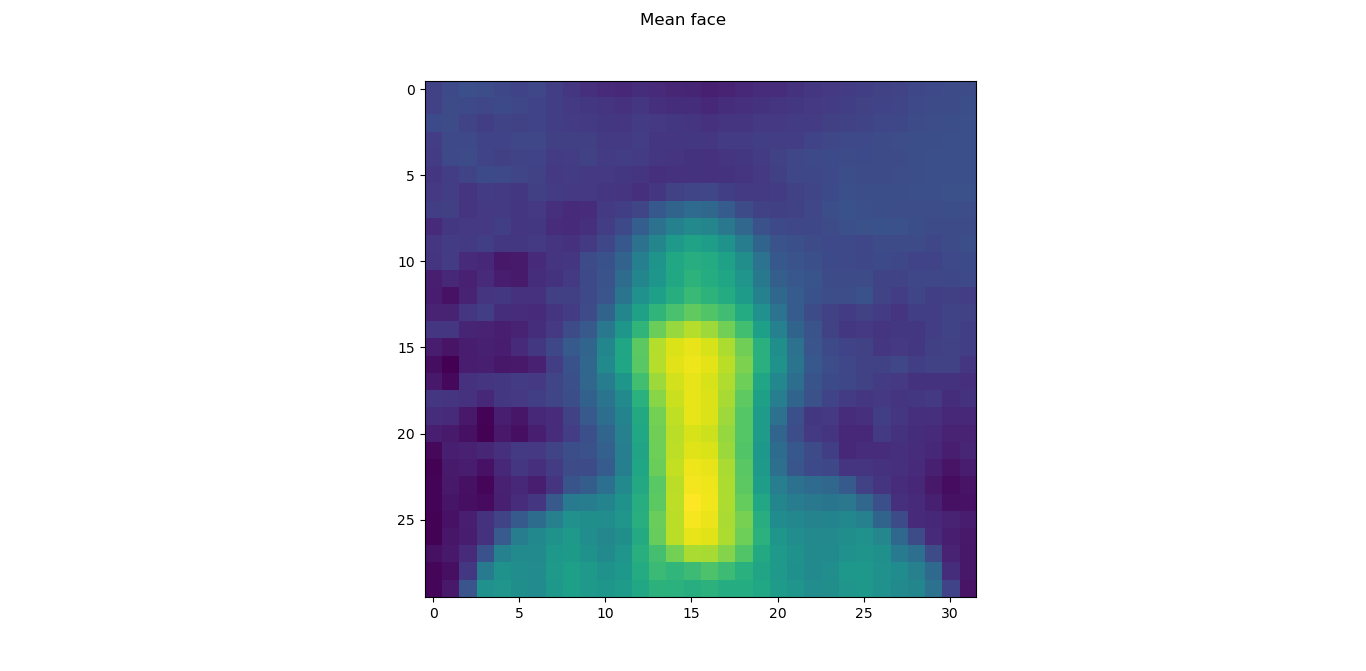
\includegraphics[scale=0.5]{mean_face}
	\caption{Mean face}
	\label{fig:mean_face}
\end{figure}
The first 5 eigen-faces are shown in Fig.\ref{fig:eig_faces}
\newpage
\begin{figure}[h!]
	\centering
	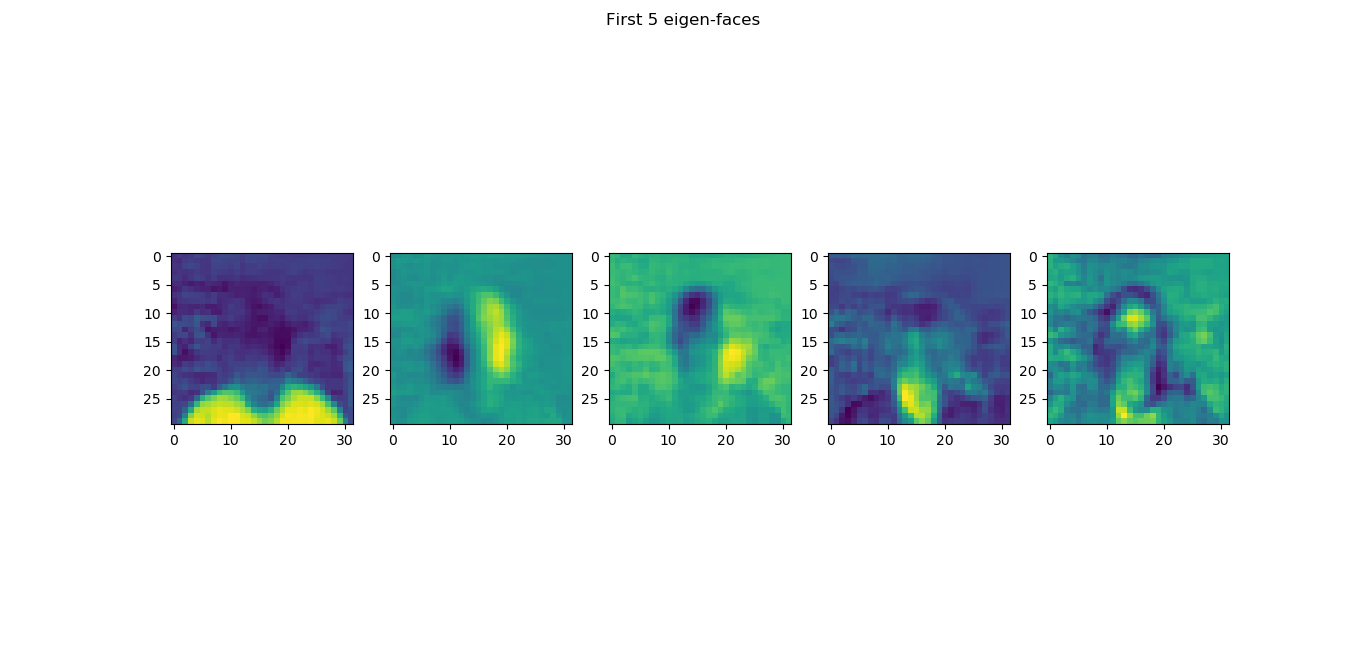
\includegraphics[scale=0.5]{eig_faces}
	\caption{First 5 eigen-faces}
	\label{fig:eig_faces}
\end{figure}
\subsection*{Solution 3.b}
We performed PCA on face training data and found the following proportion of variance plot:
\begin{figure}[h!]
	\centering
	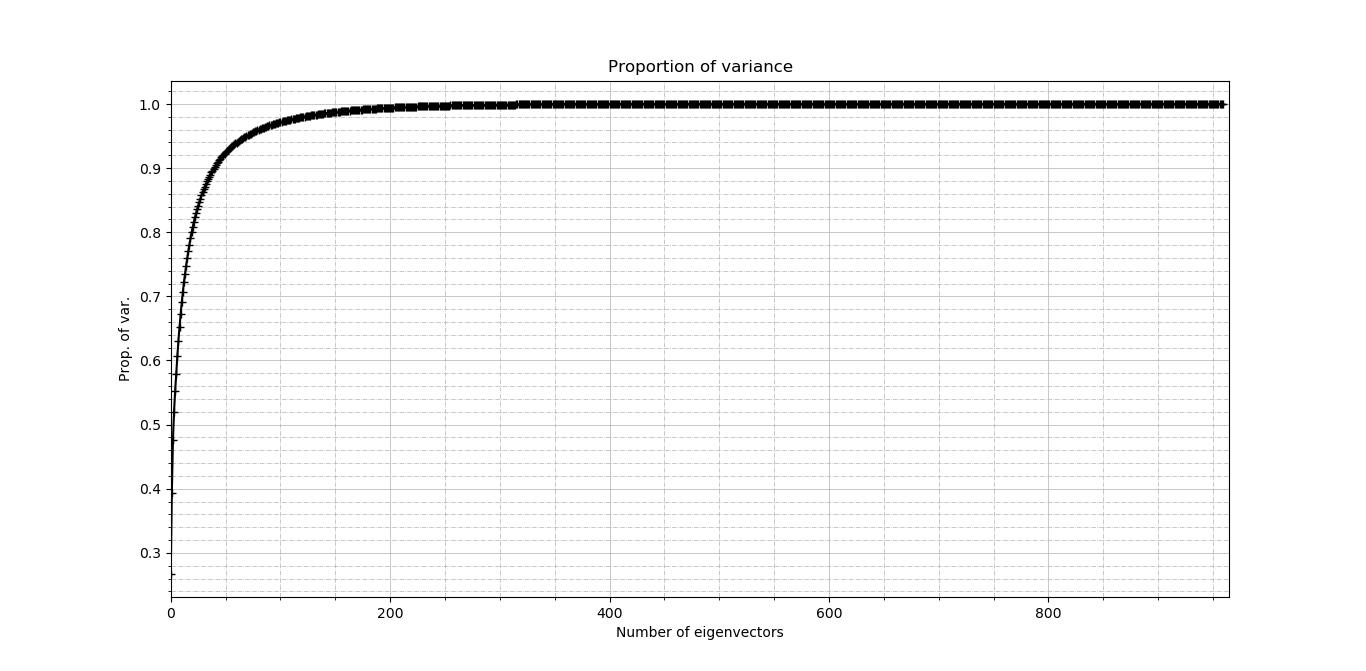
\includegraphics[scale=0.5]{pov_3b}
	\caption{Proportion of variance plot for face training data}
	\label{fig:pov_3b}
\end{figure}
\newline
We can see from Fig.\ref{fig:pov_3b} that the minimum number of eigenvectors that explain at least 90\% of the variance is 40.
\newline
Therefore, we used 40 principal components for PCA and reduced the dimension of the original face data to 40. Then, we used KNN on this reduced dimension face test data. The following table shows the error rates for different k in k-nearest neighbor algorithm on reduced face test data.
\begin{table}[h!]
	\begin{center}
		\begin{tabular}{||c | c | c | c | c ||} 
			\hline
			k & 1 & 3 & 5 & 7 \\ [0.5ex] 
			\hline\hline
			Error rate(\%) & 10.483 & 24.193 & 39.516 & 39.516 \\ [1ex]
			\hline
		\end{tabular}
	\end{center}
	\caption{Q3.b: Error-rate Vs. k table}
\end{table}
\subsection*{Solution 3.c}
\begin{figure}[h!]
	\centering
	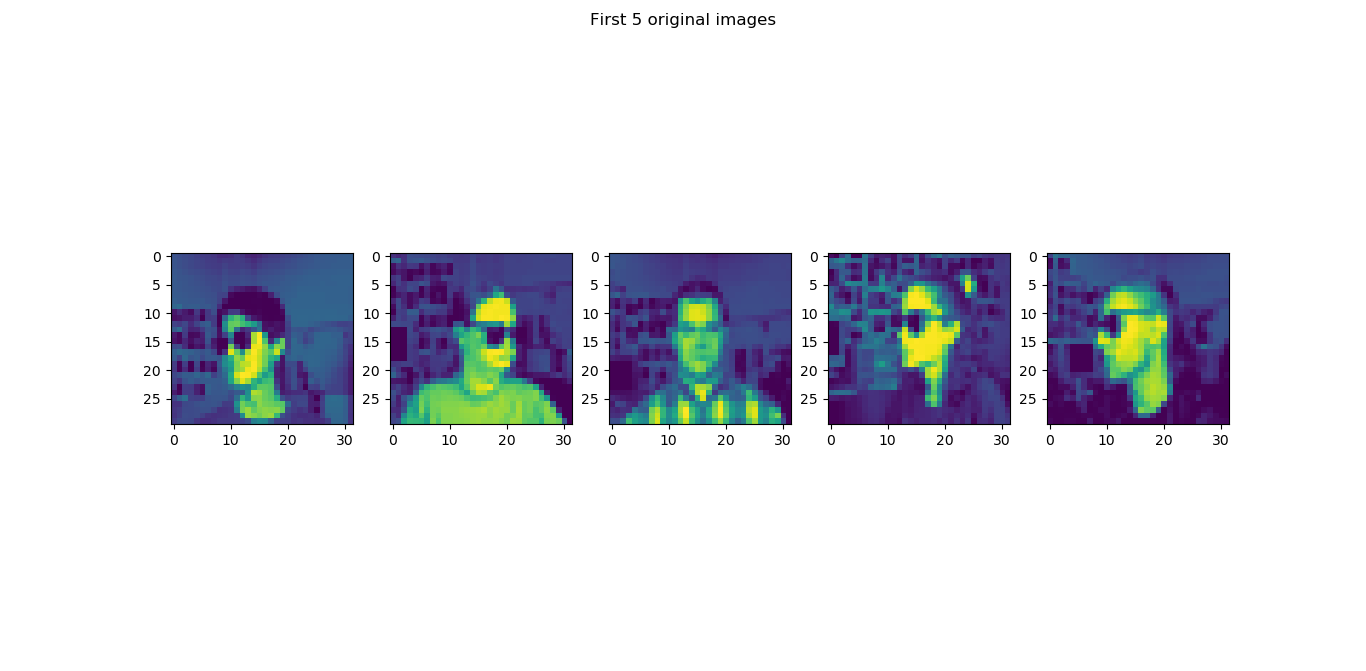
\includegraphics[scale=0.5]{face_orig}
	\caption{Original first 5 faces from training data}
	\label{fig:face_orig}
\end{figure}
\begin{figure}[h!]
	\centering
	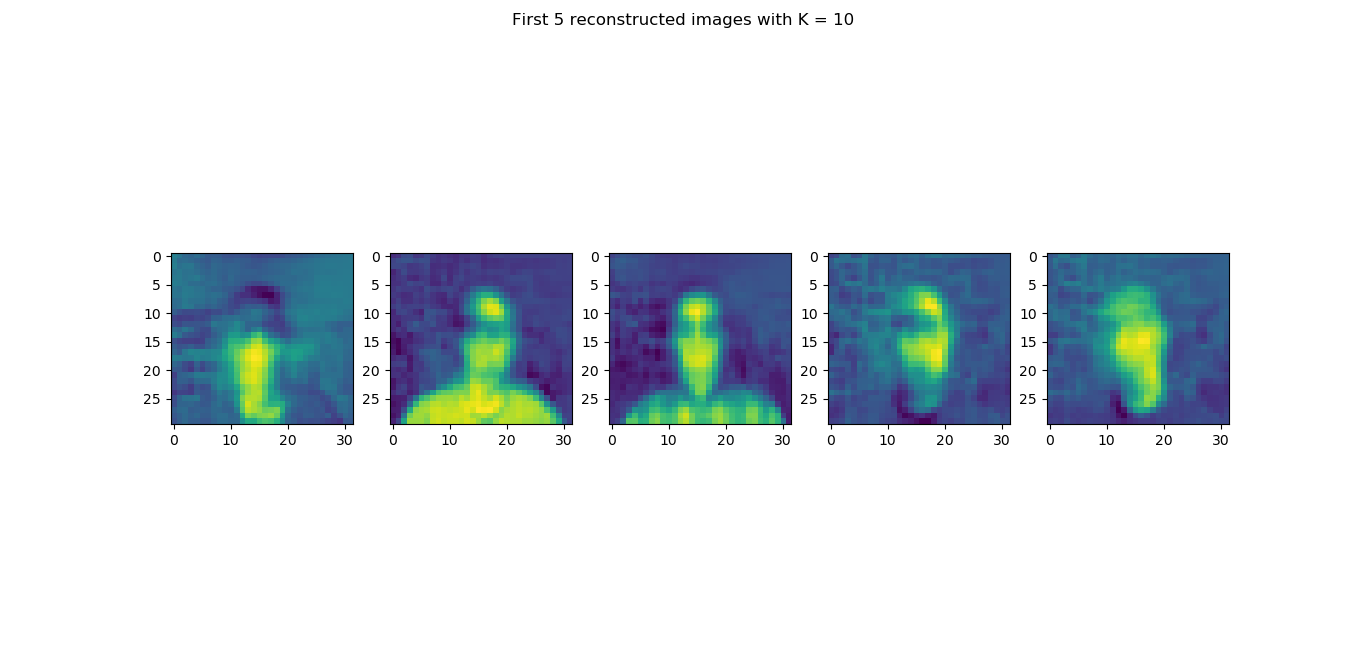
\includegraphics[scale=0.5]{face_pca_10}
	\caption{First 5 reconstructed faces using 10 principal components}
	\label{fig:face_pca_10}
\end{figure}
\begin{figure}[h!]
	\centering
	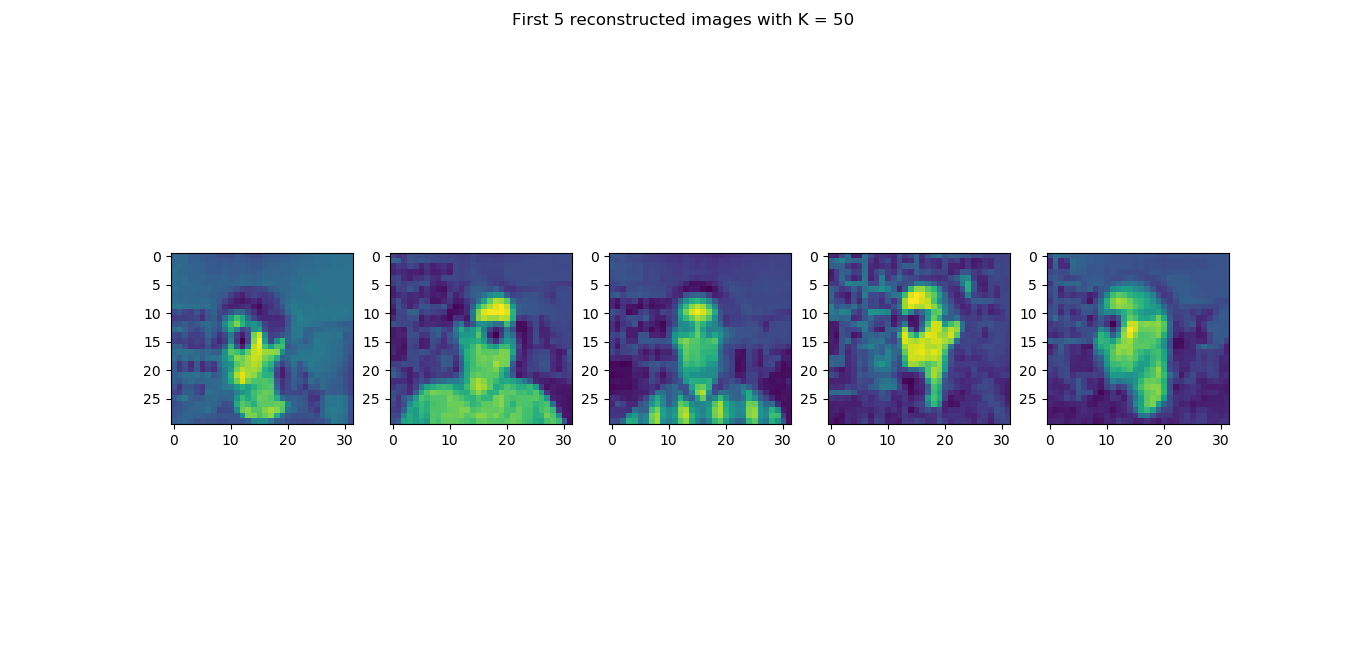
\includegraphics[scale=0.5]{face_pca_50}
	\caption{First 5 reconstructed faces using 50 principal components}
	\label{fig:face_pca_50}
\end{figure}
\begin{figure}[h!]
	\centering
	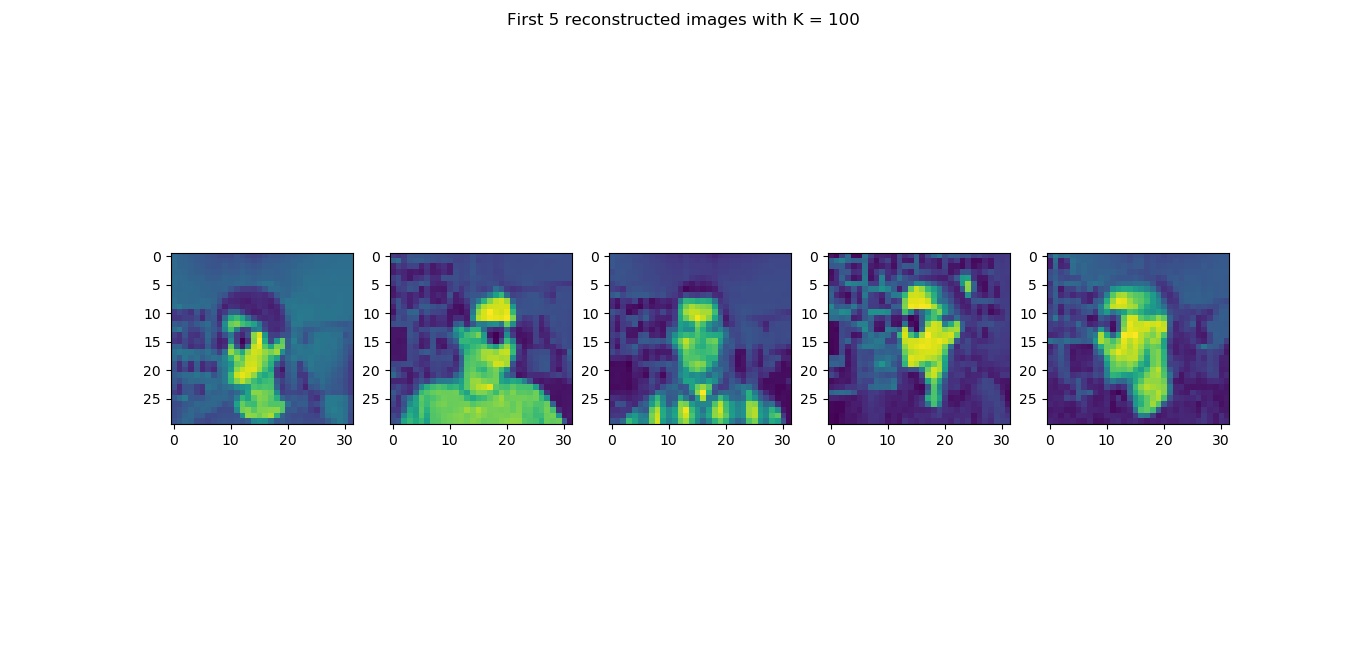
\includegraphics[scale=0.5]{face_pca_100}
	\caption{First 5 reconstructed faces using 100 principal components}
	\label{fig:face_pca_100}
\end{figure}
\newpage
Thus we can see that as we increase the number of principal components, reconstructed images become closer to the original images but at a cost of increased complexity and processing time.